% We use two main columns for the whole page layout
%\setcolumnsep{10pt} % Space between the text and the images
\columnratio{0.5}

\begin{paracol}{2}
  %% --- LEFT COLUMN: YOUR TEXT ---
  \section*{Introduction}

  The assignment provides data on the glucose metabolism measurements
  taken from isthmuscingulate and precuneus regions on the brain as a possible
  measurement to diagnose dementia of Alzheimer's type (DAT), labeled sDAT/1.
  The data on healthy individuals (NC) is labeled sNC/0 on the report.
  The data was proved in two groups - The training data, and the test data,
  used in their respective functions.

  With this data, we implemented studied the implementation of a Nearest Neighbor classifier
  using various number of neighbors ($k$) and metrics to evaluate the performance in the context of
  over/under fitting, bias and variance.

  The code was implemented using the python library \textit{scikit-learn 1.8.0}
  for the classifier and accuracy scores, the \textit{pandas 2.3.3} for data handling,
  and \textit{matplotlib 3.10.8} for plotting.


  \section*{Question 1}

  The first group Nearest Neighbors classifiers (refereed from now on as kNN) uses the \textit{Euclidean}
  for values of k=1, 3, 5, 10, 20, 30, 50, 100, 150, 200.
  The resulting boundary regions overlaid with
  the training and testing data are presented in figures \ref{fig:Q1k1} to \ref{fig:Q1k200}, the training
  and test error for each value of k is presented in the table \ref{tab:Q1errors}.
  
  
  \begin{table}[t!]
    \begin{tabular}{lll}
      k   & Training Error & Testing Error \\
      1   & 0              & 0.220         \\
      3   & 0.143          & 0.205         \\
      5   & 0.156          & 0.170         \\
      10  & 0.152          & 0.170         \\
      20  & 0.169          & 0.170         \\
      \textbf{ 30}  & \textbf{0.169}          & \textbf{0.160}         \\
      50  & 0.158          & 0.190         \\
      100 & 0.196          & 0.200         \\
      150 & 0.192          & 0.190         \\
      200 & 0.222          & 0.205        
    \end{tabular}
    \caption{Training and error rate of kNN classifiers for $k = 1,3,5,10,20,30,50,100,150,200$}
    \label{tab:Q1errors}
  \end{table}


  The \textbf{best performance} for this metric is obtained for $k=30$ neighbors, with a testing
  error of $0.170$, beating the performance of the other kNN classifiers by at least $5\%$.
  Other \textbf{intermediate values} of k ($k=5, 10$ and $20$) also
  performed well when in comparison to the best performing model ($k=30$).

  For the \textbf{low values} of k, the testing error was  25\% higher for $k=3$,
  and 37.5\% higher for k=1. This is the result of
  \textbf{over fitting}, as the capacity of the kNN classifier \textbf{increases} as k \textbf{decreases}.
  This is specially notable for the k=1 case, where each point is it's own closest neighbor, as a result
  it can fit any dataset with training error of 0, even if the generalized error is high, indicating that low
  values of k are unable to perform good predictions on unseen data. In term of bias and variance,
  low values of k have \textbf{low bias}, as they can easily conform to any data set, while having
  \textbf{high variance}, as different datasets with generate significantly different models.

  For the \textbf{high values} of k, the testing error was also over 20\% worse then the best
  performing classifier, but for different reasons than the low value case. For high values of
  k, the model capacity \textbf{decreases}. For example, in the extreme where k is equal in size to the
  dataset, a kNN classifier will classify any point was the majority class, due to it counting
  every point as a neighbor.

  Even before this extreme scenario, it's possible to see the increase in bias of the model
  as k increases. For low values of k, the boundary regions are highly non-linear and discontinuous,
  this also represents well the high variance of low k kNN classifiers, as a different dataset would result
  in a significantly different boundary region.
  As k increases, the boundary between the sNC and sDAT regions becomes more \textit{``well-behaved''}.
  In intermediate values of k, the non-linear behavior is enough to differentiates classes in the
  region where the sNC and sDAT data set mixes, but not too much to over fit the training data.
  And for high values k, the bias is too high, and the boundary becomes basically a straight line
  separating the regions with the majority of each class, so even a different dataset would still
  generate a similar boundary region, as the kNN classifier is low variance for high values of k. The best
  scenario within the values of k provided is k=30, for a generalization error of $0.169$.

  \renewcommand{\thefigure}{6}
  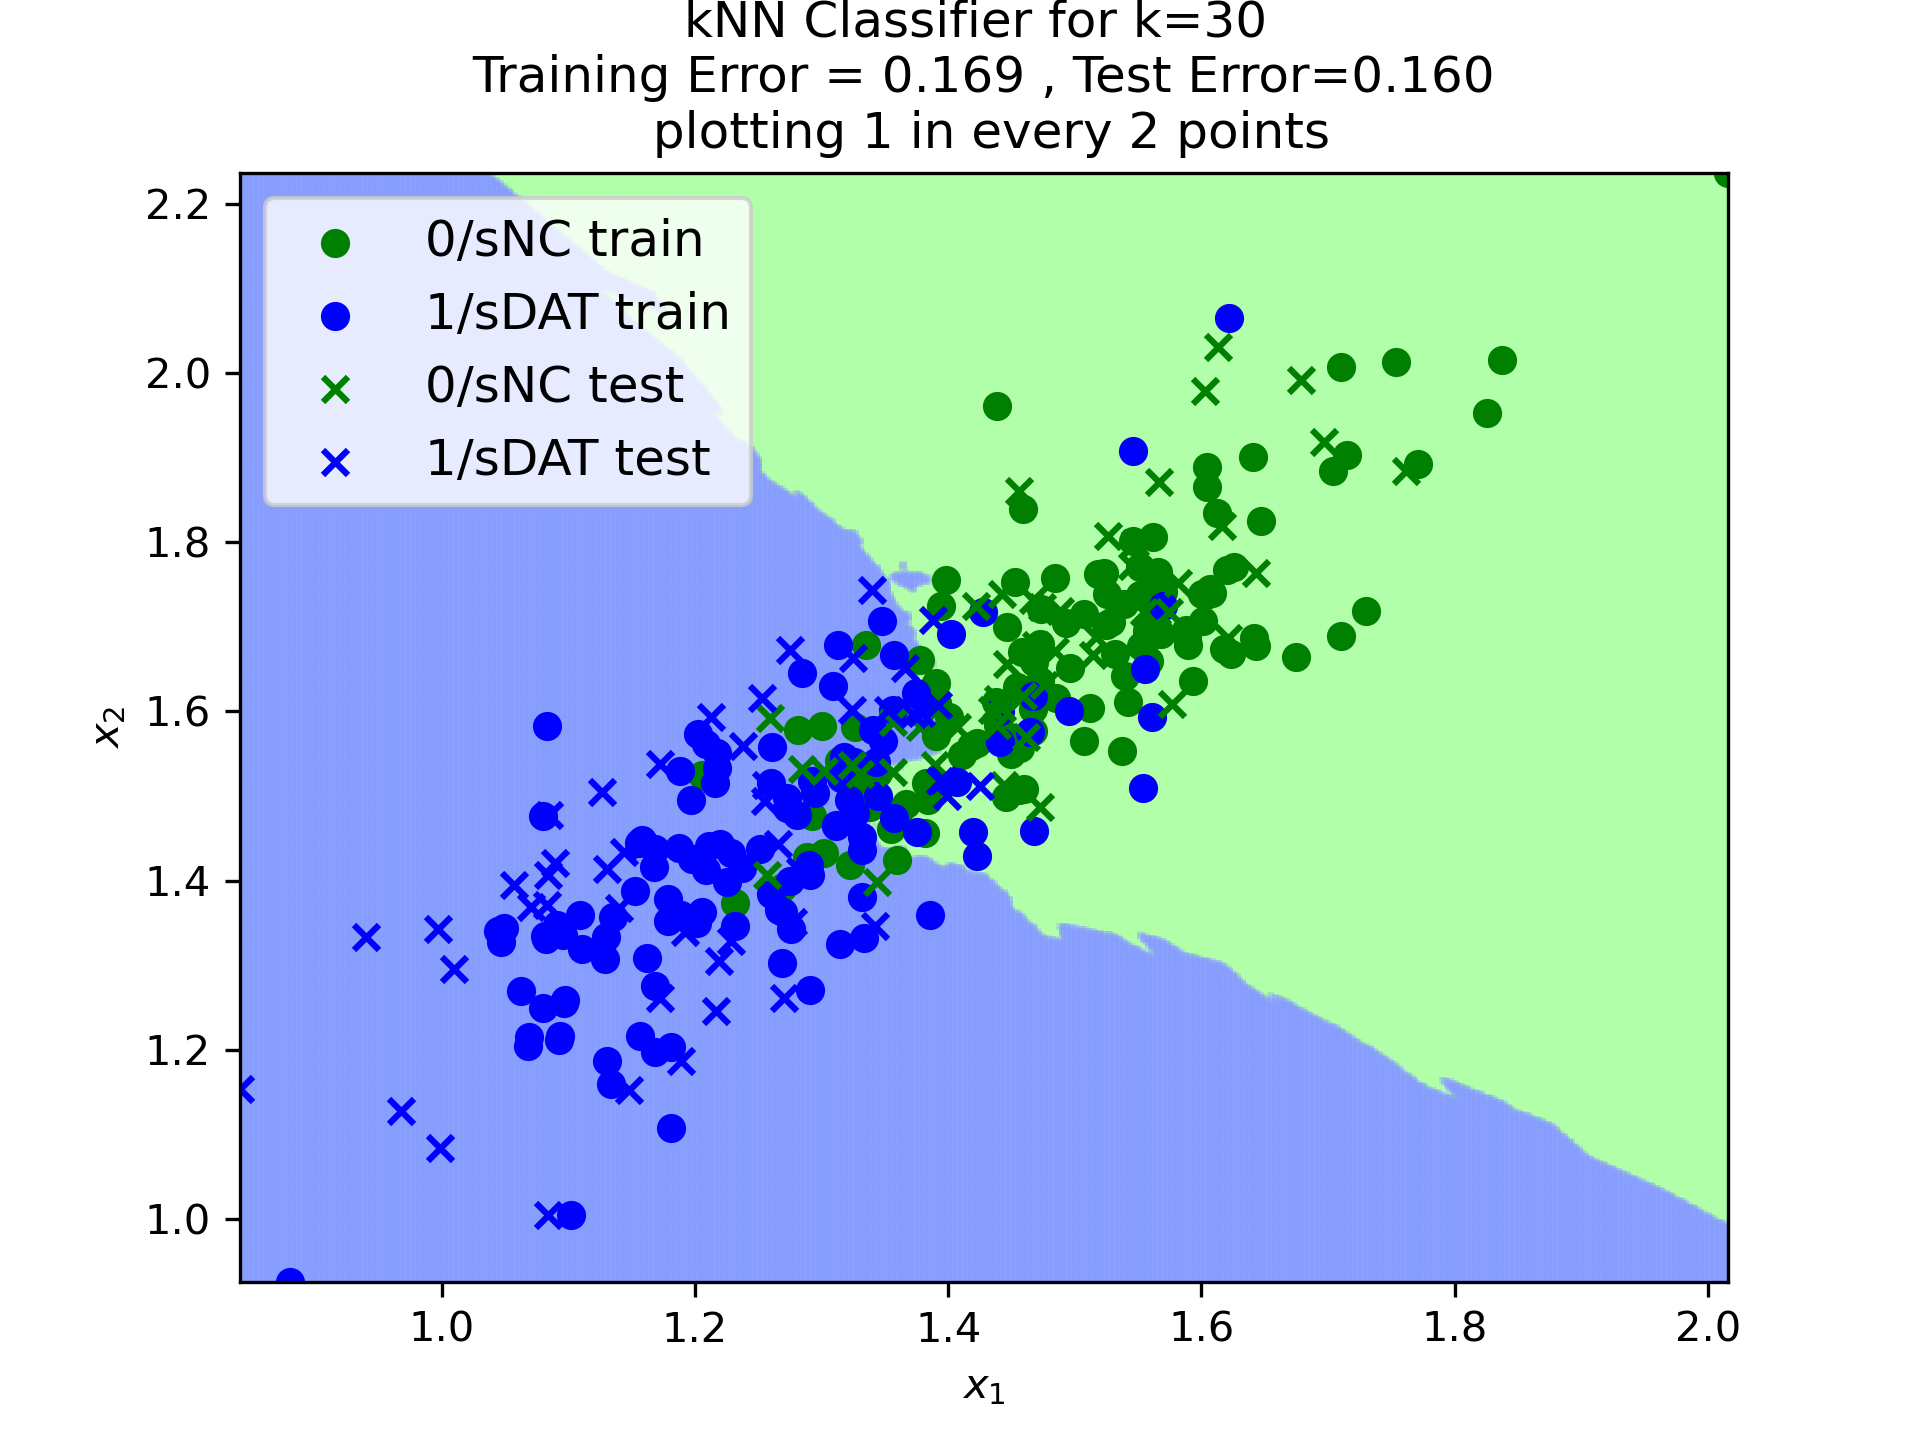
\includegraphics[width=0.95\linewidth]{Graphs/Q1_k30.png}
  \captionof{figure}{Nearest Neighbor classifier for k = 30 with sDAT region in blue and sNC region colored green, with training and test data overlayed}
  \label{fig:Q1k30}
  \vspace{20pt}

  \renewcommand{\thefigure}{8}
  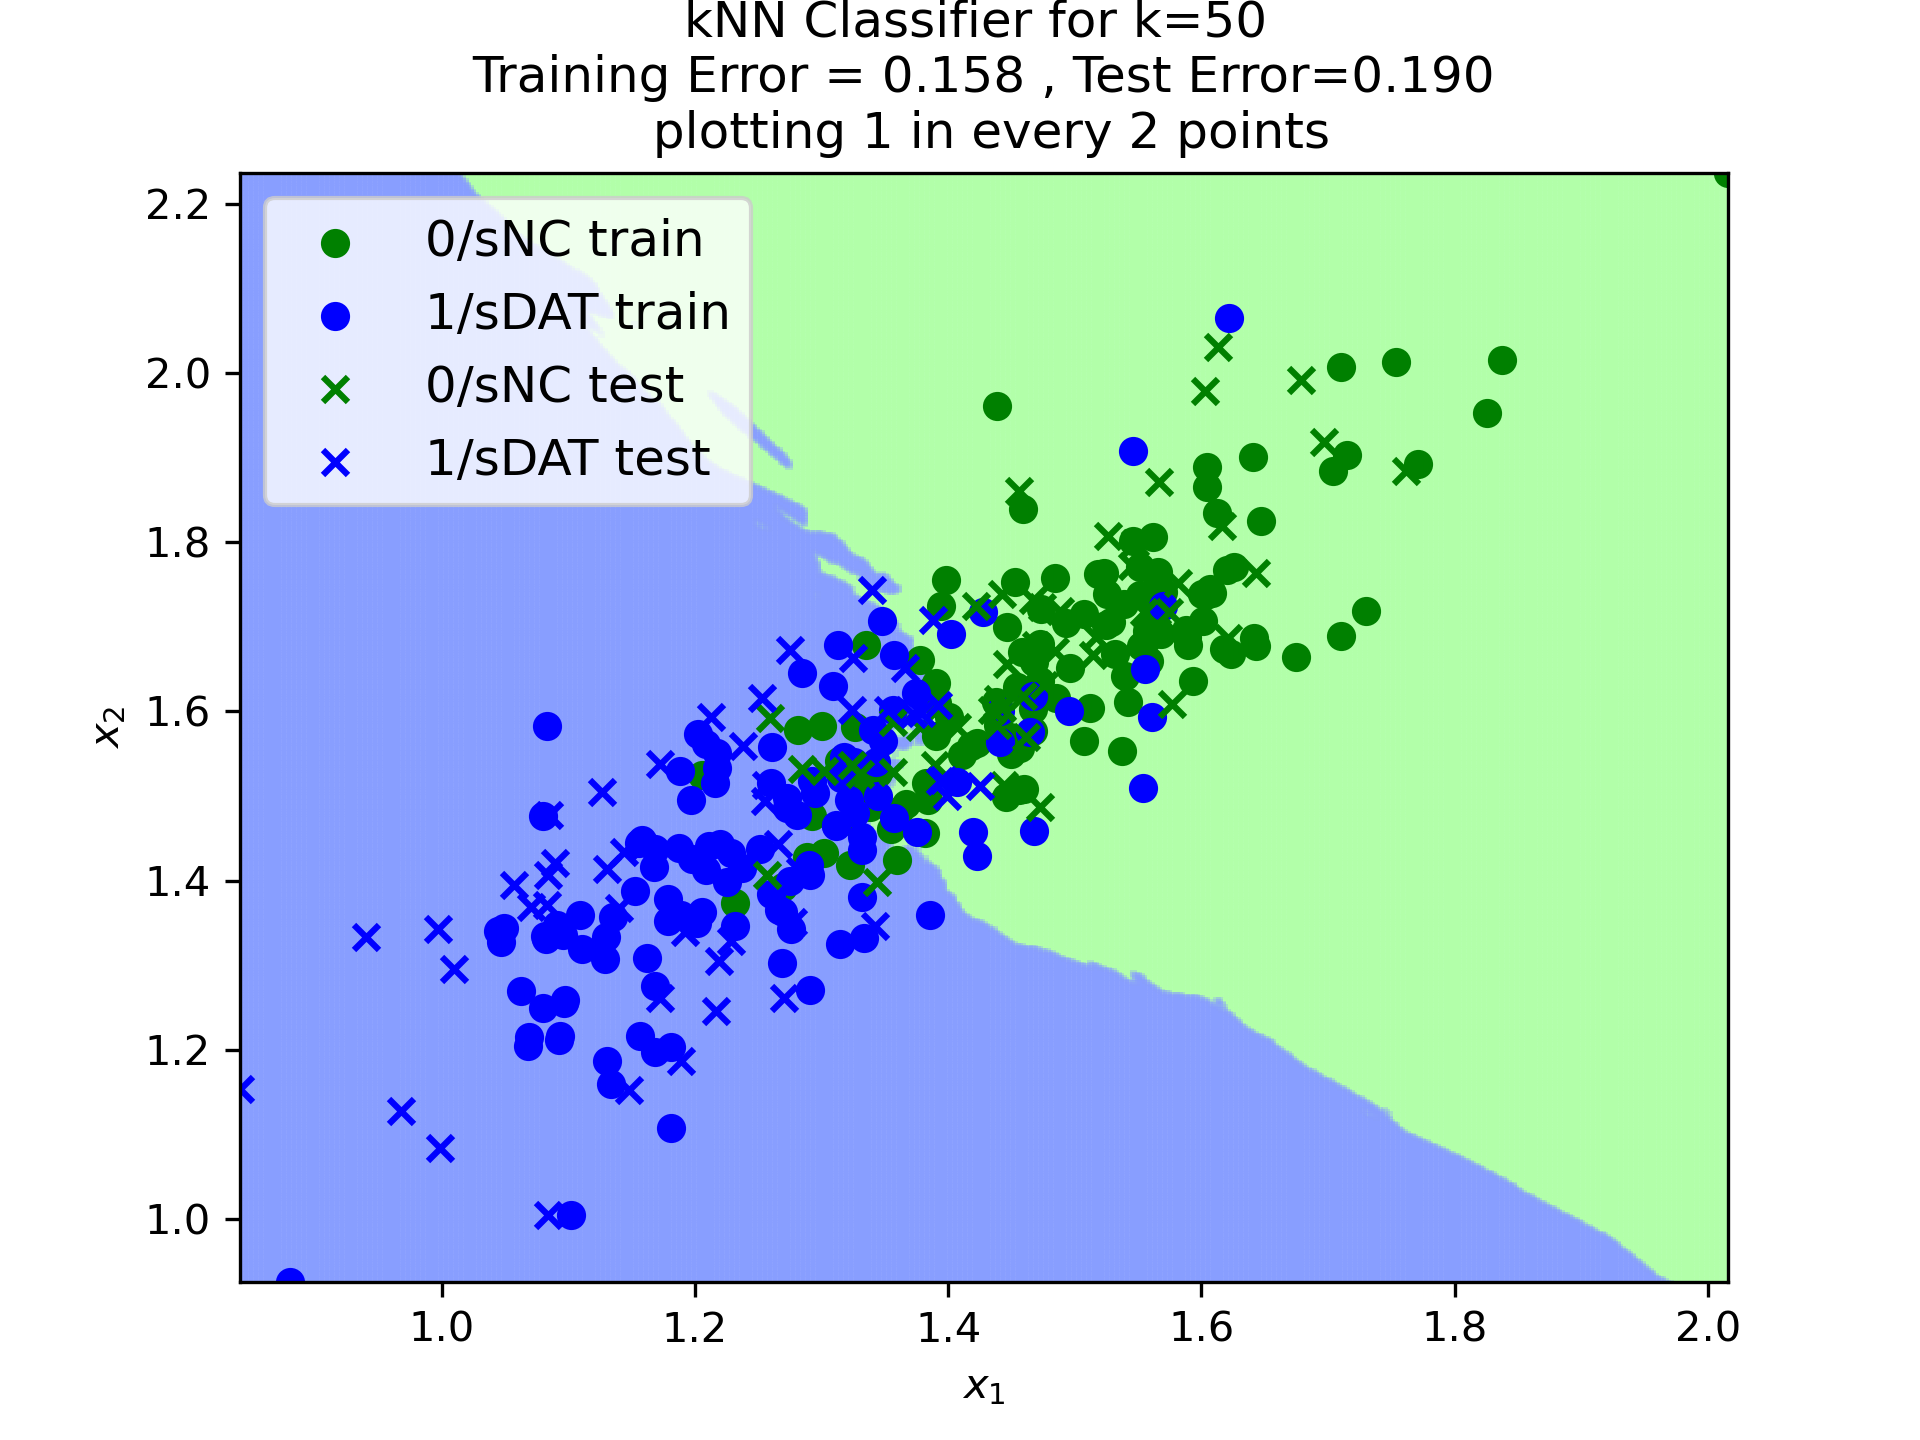
\includegraphics[width=0.95\linewidth]{Graphs/Q1_k50.png}
  \captionof{figure}{Nearest Neighbor classifier for k = 50 with sDAT region in blue and sNC region colored green, with training and test data overlayed}
  \label{fig:Q1k50}
  \vspace{20pt}

  
  \renewcommand{\thefigure}{10}
  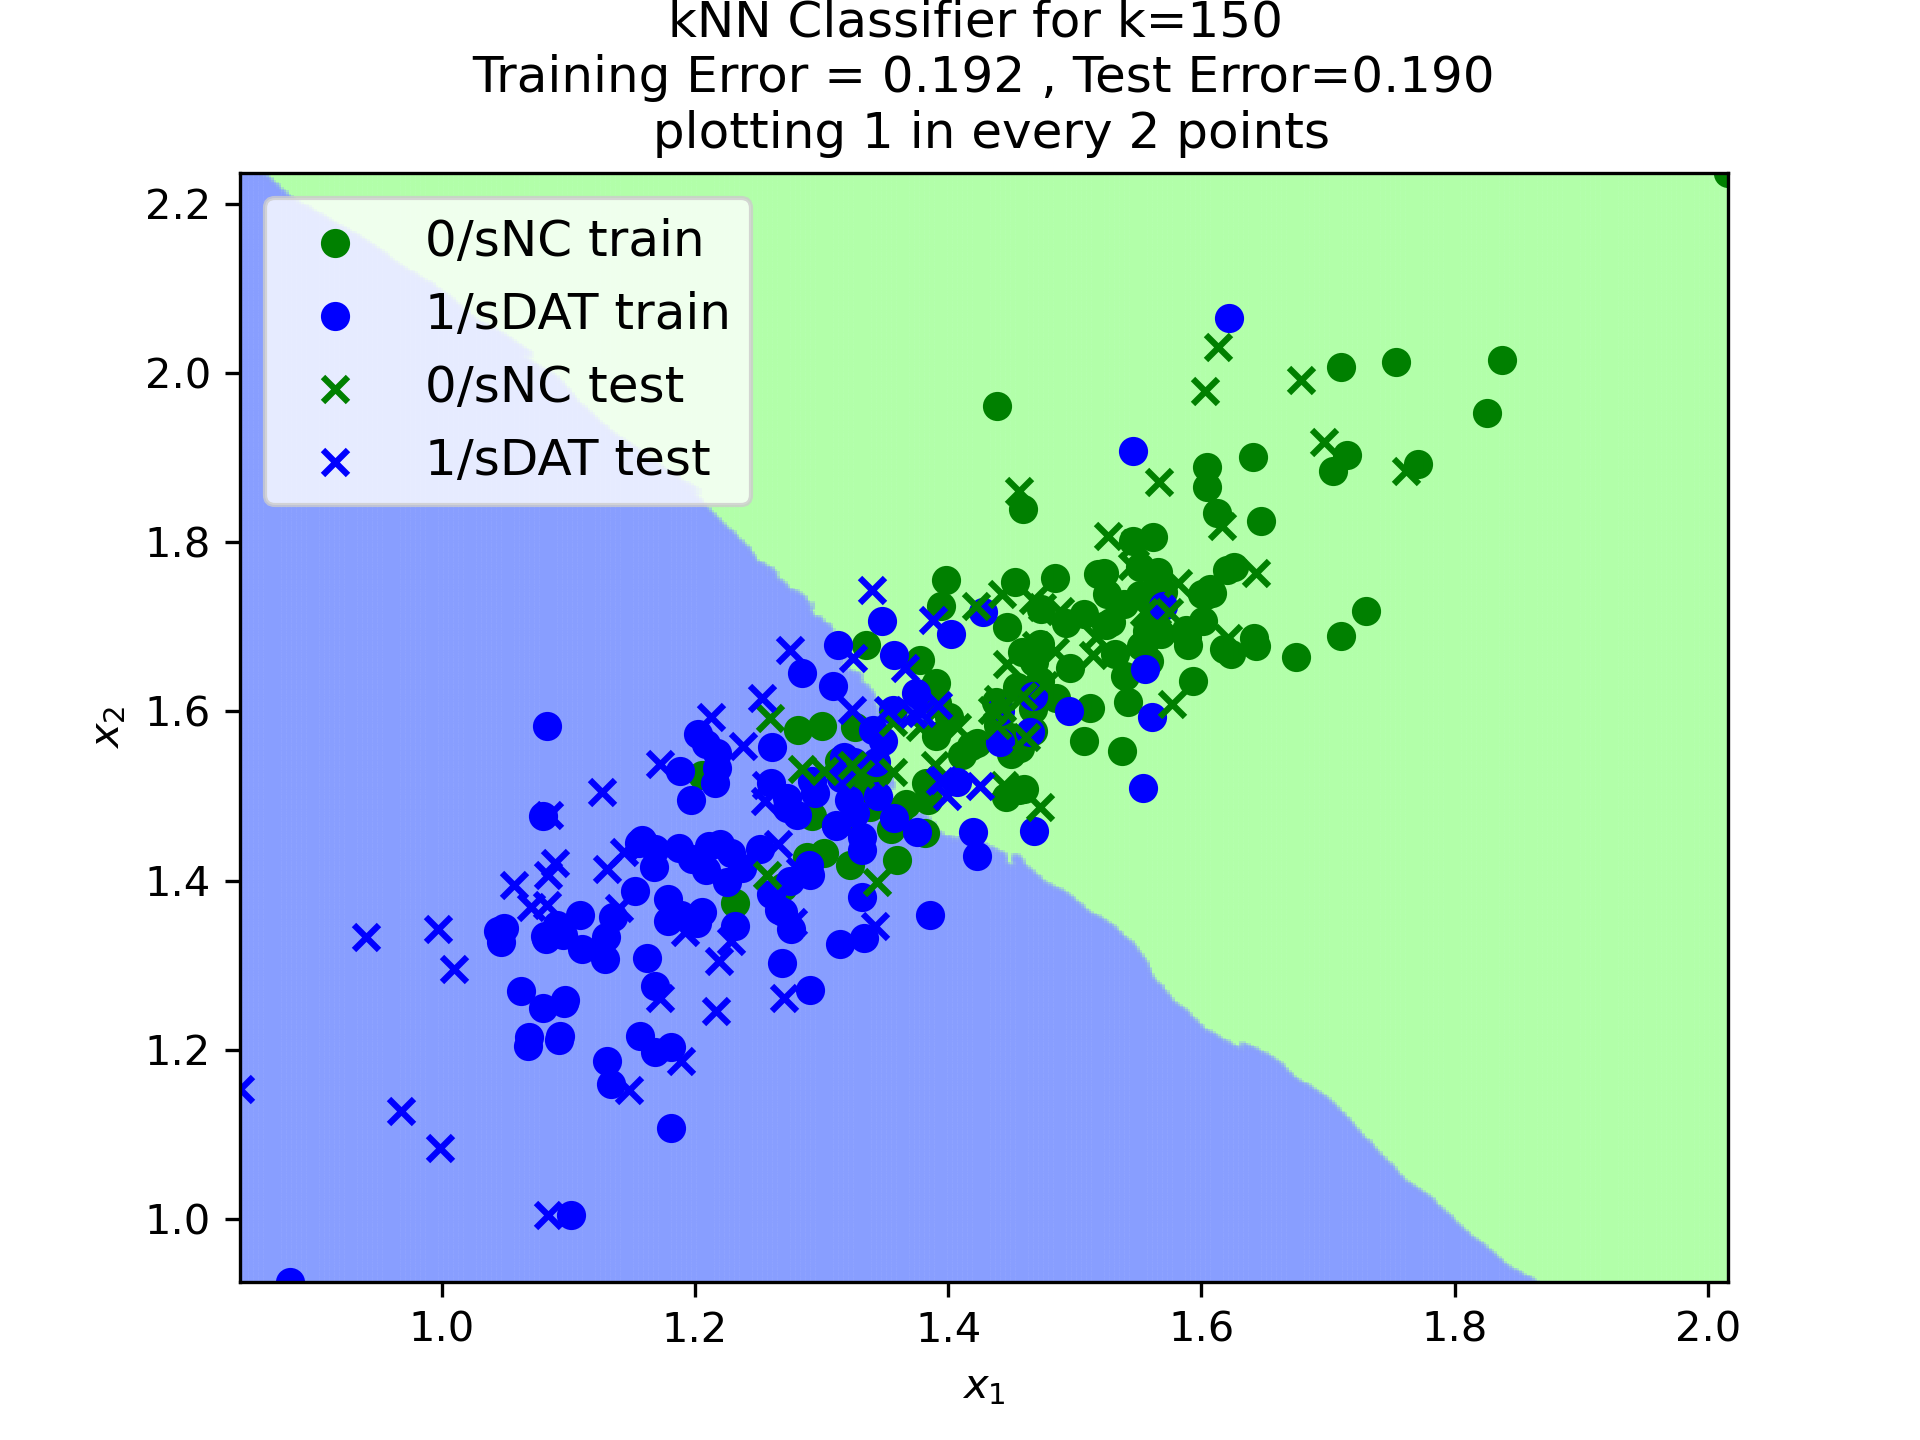
\includegraphics[width=0.95\linewidth]{Graphs/Q1_k150.png}
  \captionof{figure}{Nearest Neighbor classifier for k = 150 with sDAT region in blue and sNC region colored green, with training and test data overlayed}
  \label{fig:Q1k150}
  \vspace{20pt}


  
  %% --- SWITCH TO RIGHT COLUMN ---
  \switchcolumn
  %\subsection*{kNN Classifier Boundary Regions for Q1}


  
  \centering

  \renewcommand{\thefigure}{1}
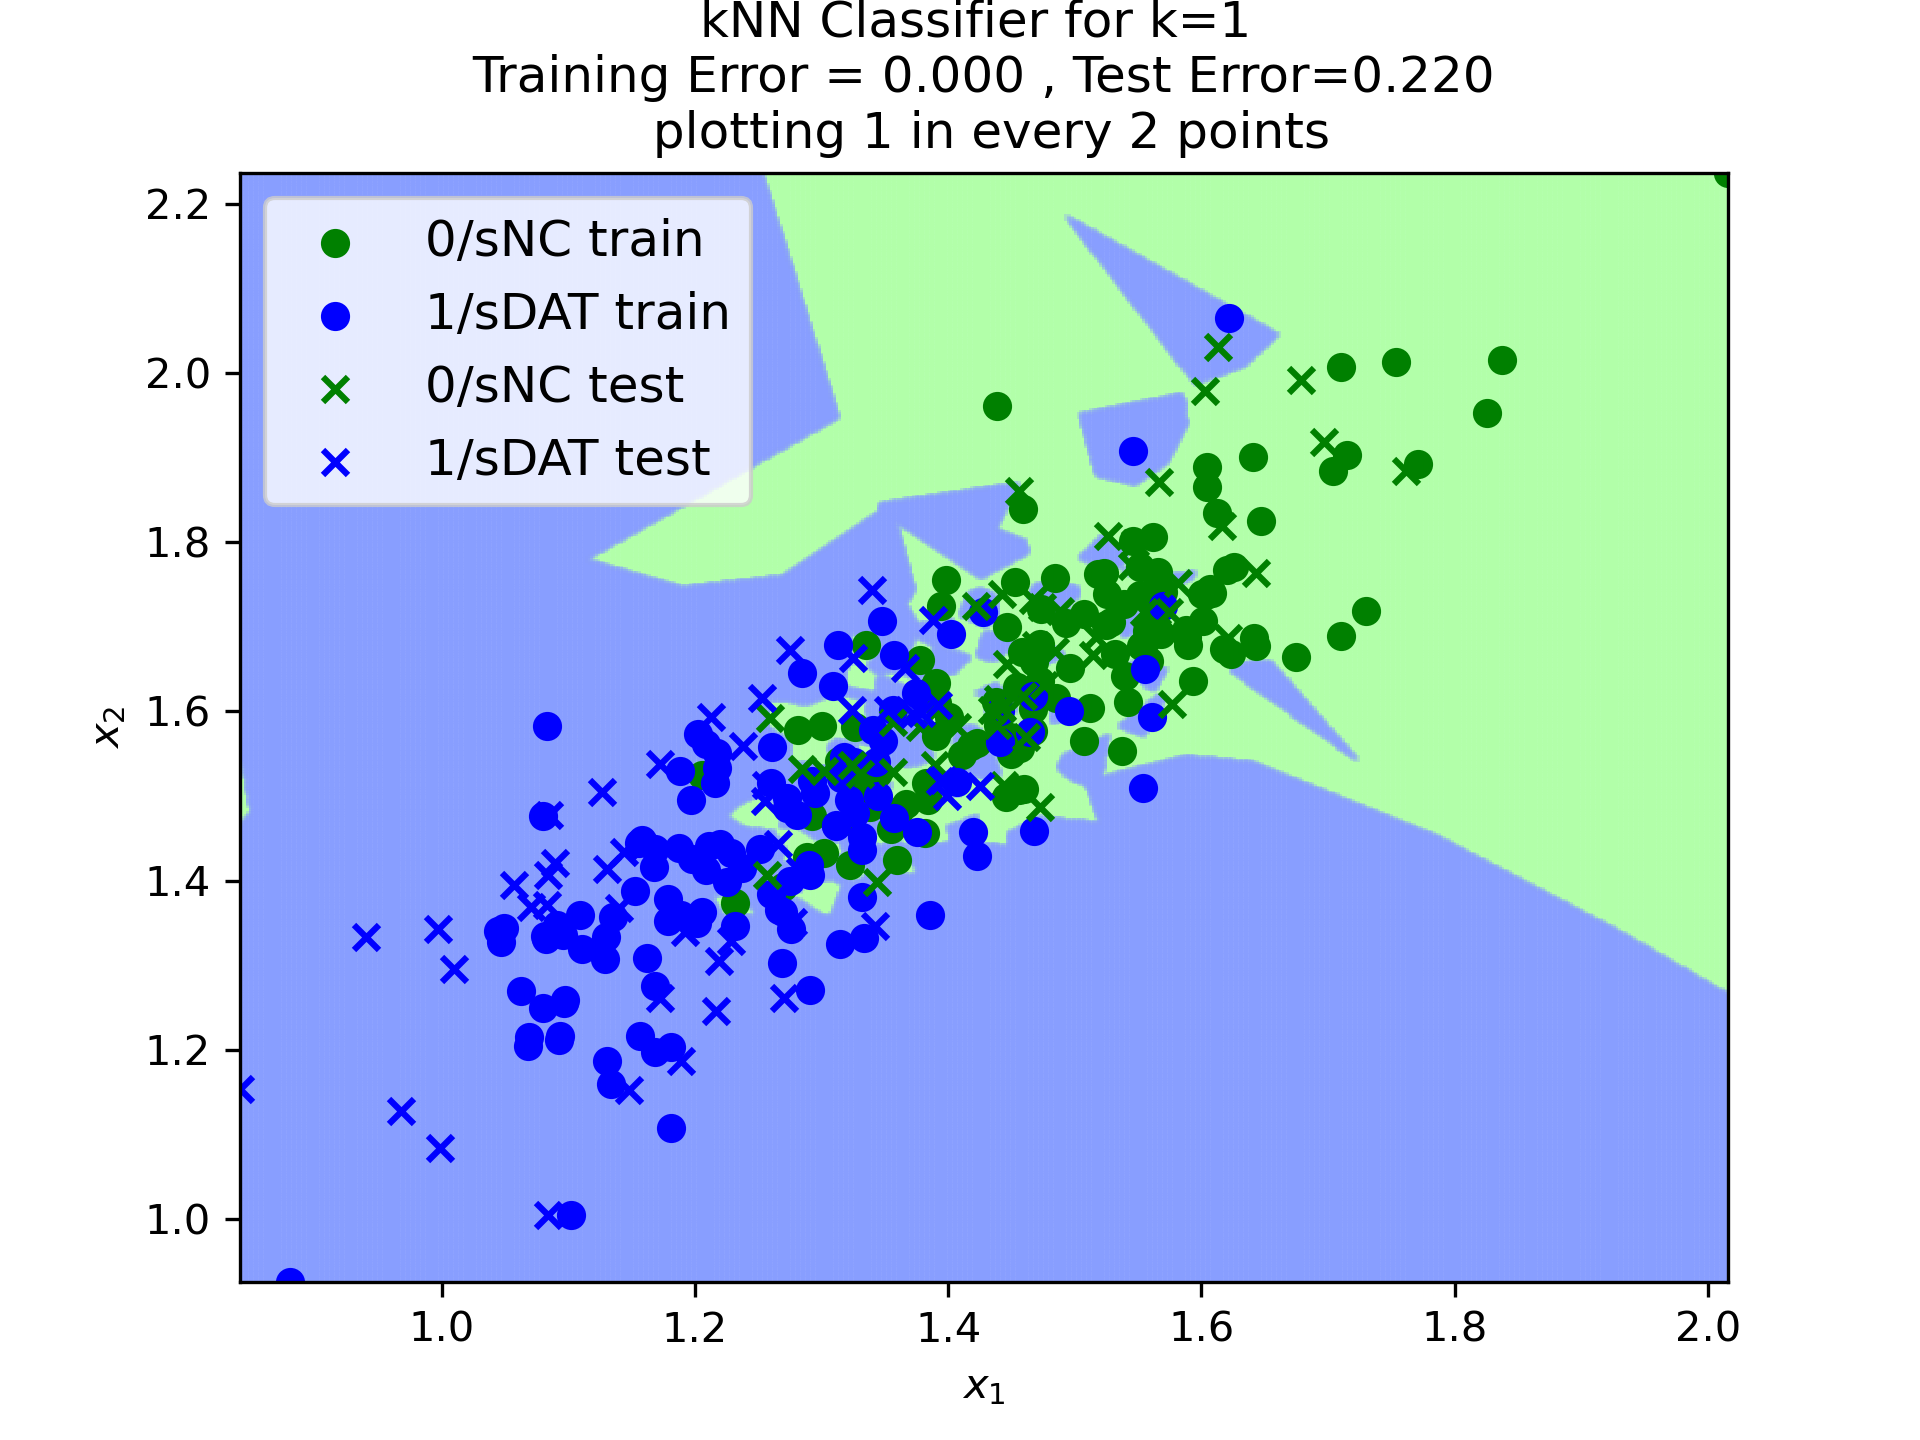
\includegraphics[width=0.95\linewidth]{Graphs/Q1_k1.png}
\captionof{figure}{Nearest Neighbor classifier for k = 1 with sDAT region in blue and sNC region colored green, with training and test data overlayed}
\label{fig:Q1k1}
\vspace{20pt}

\renewcommand{\thefigure}{2}
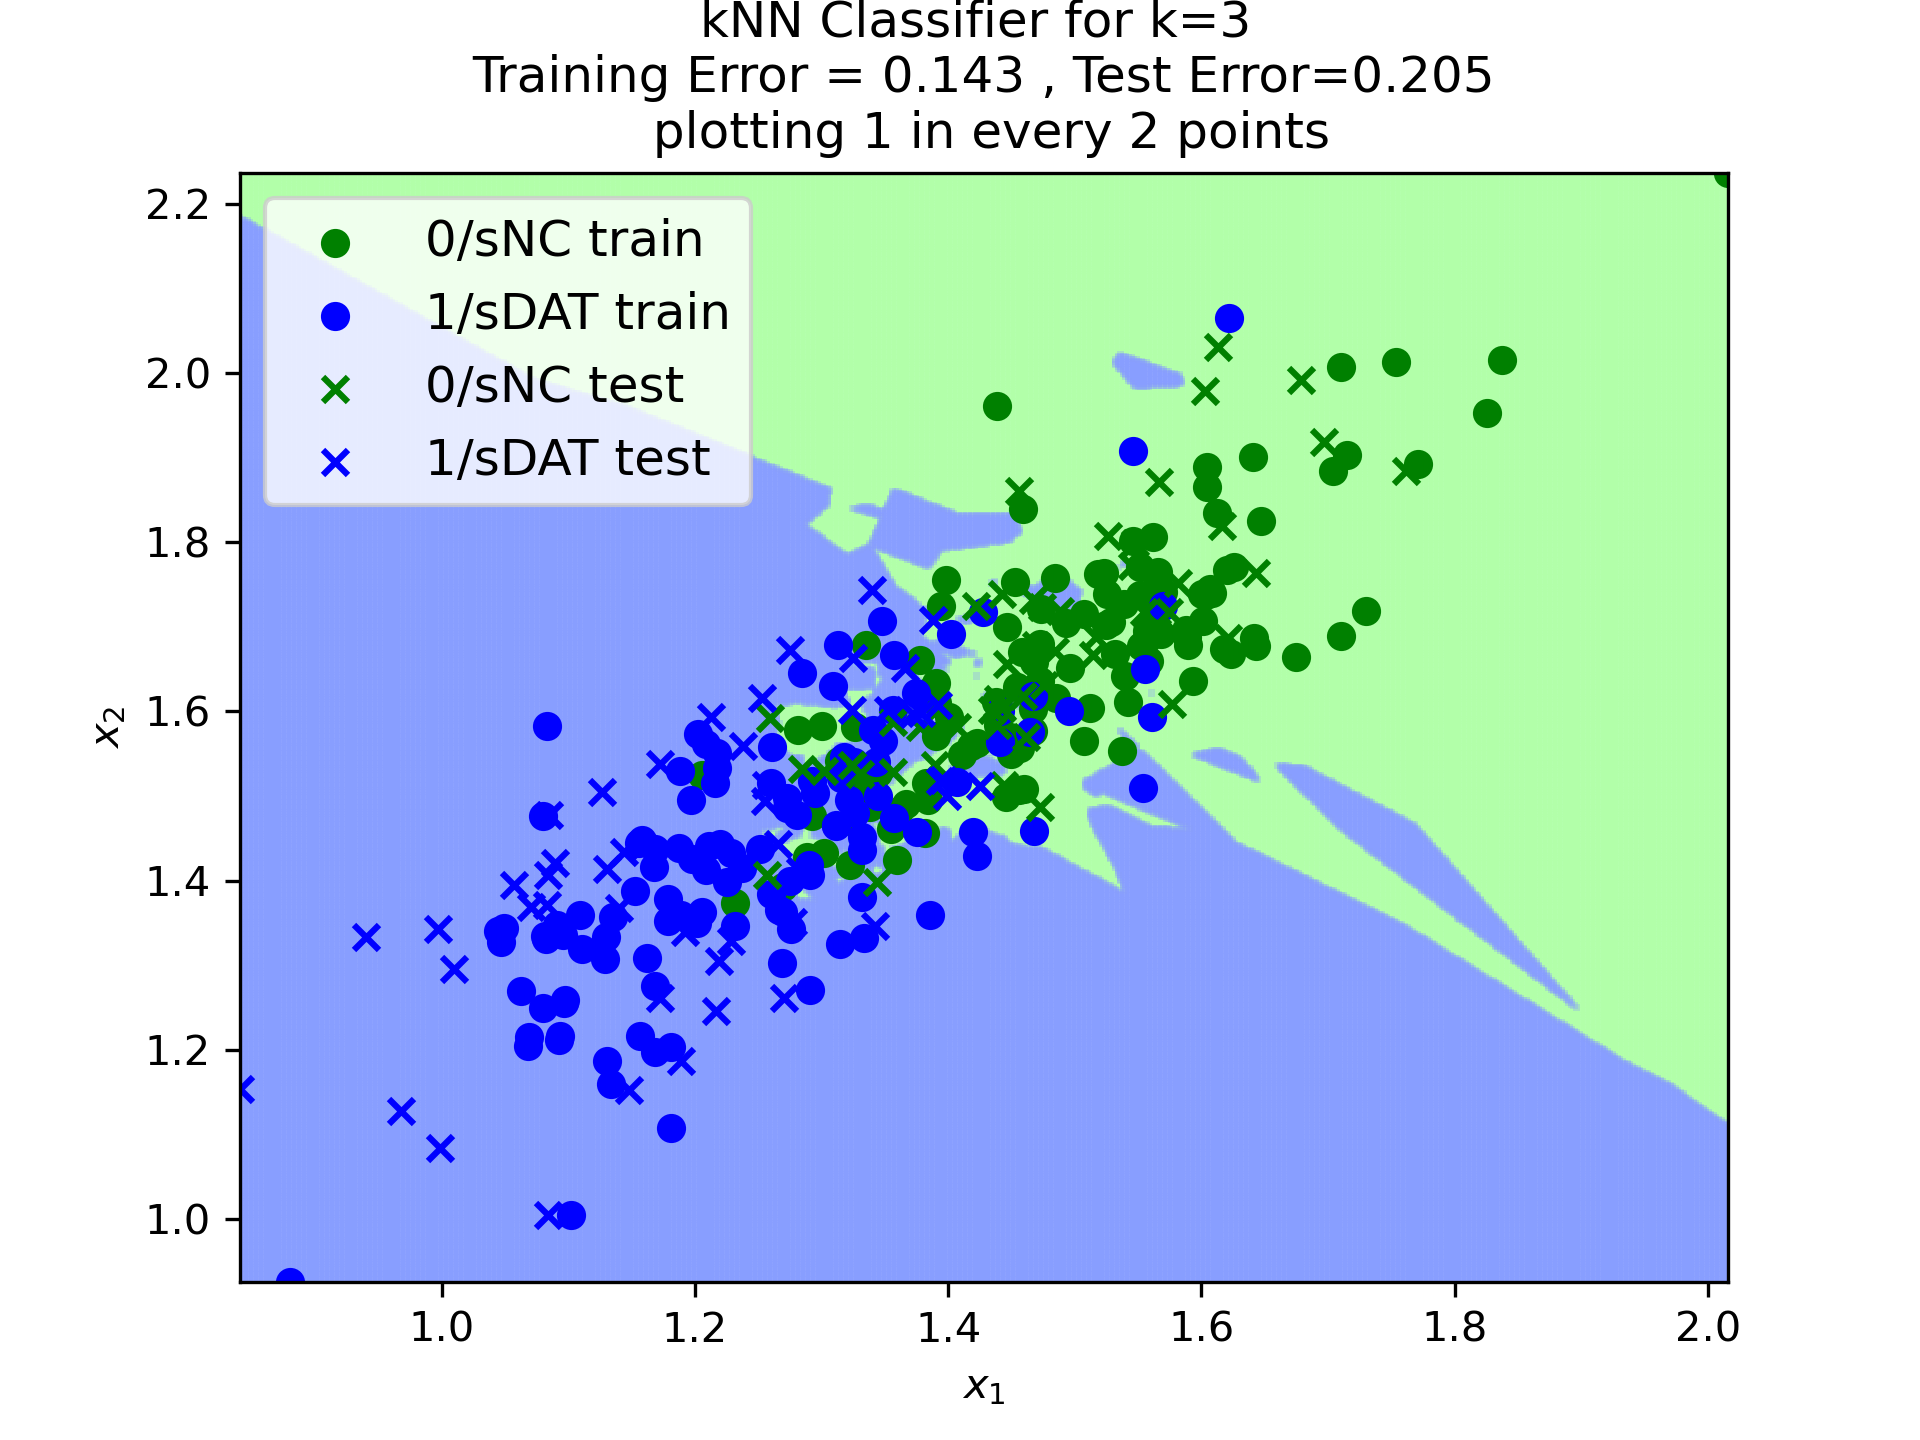
\includegraphics[width=0.95\linewidth]{Graphs/Q1_k3.png}
\captionof{figure}{Nearest Neighbor classifier for k = 3 with sDAT region in blue and sNC region colored green, with training and test data overlayed}
\label{fig:Q1k3}
\vspace{20pt}

\renewcommand{\thefigure}{3}
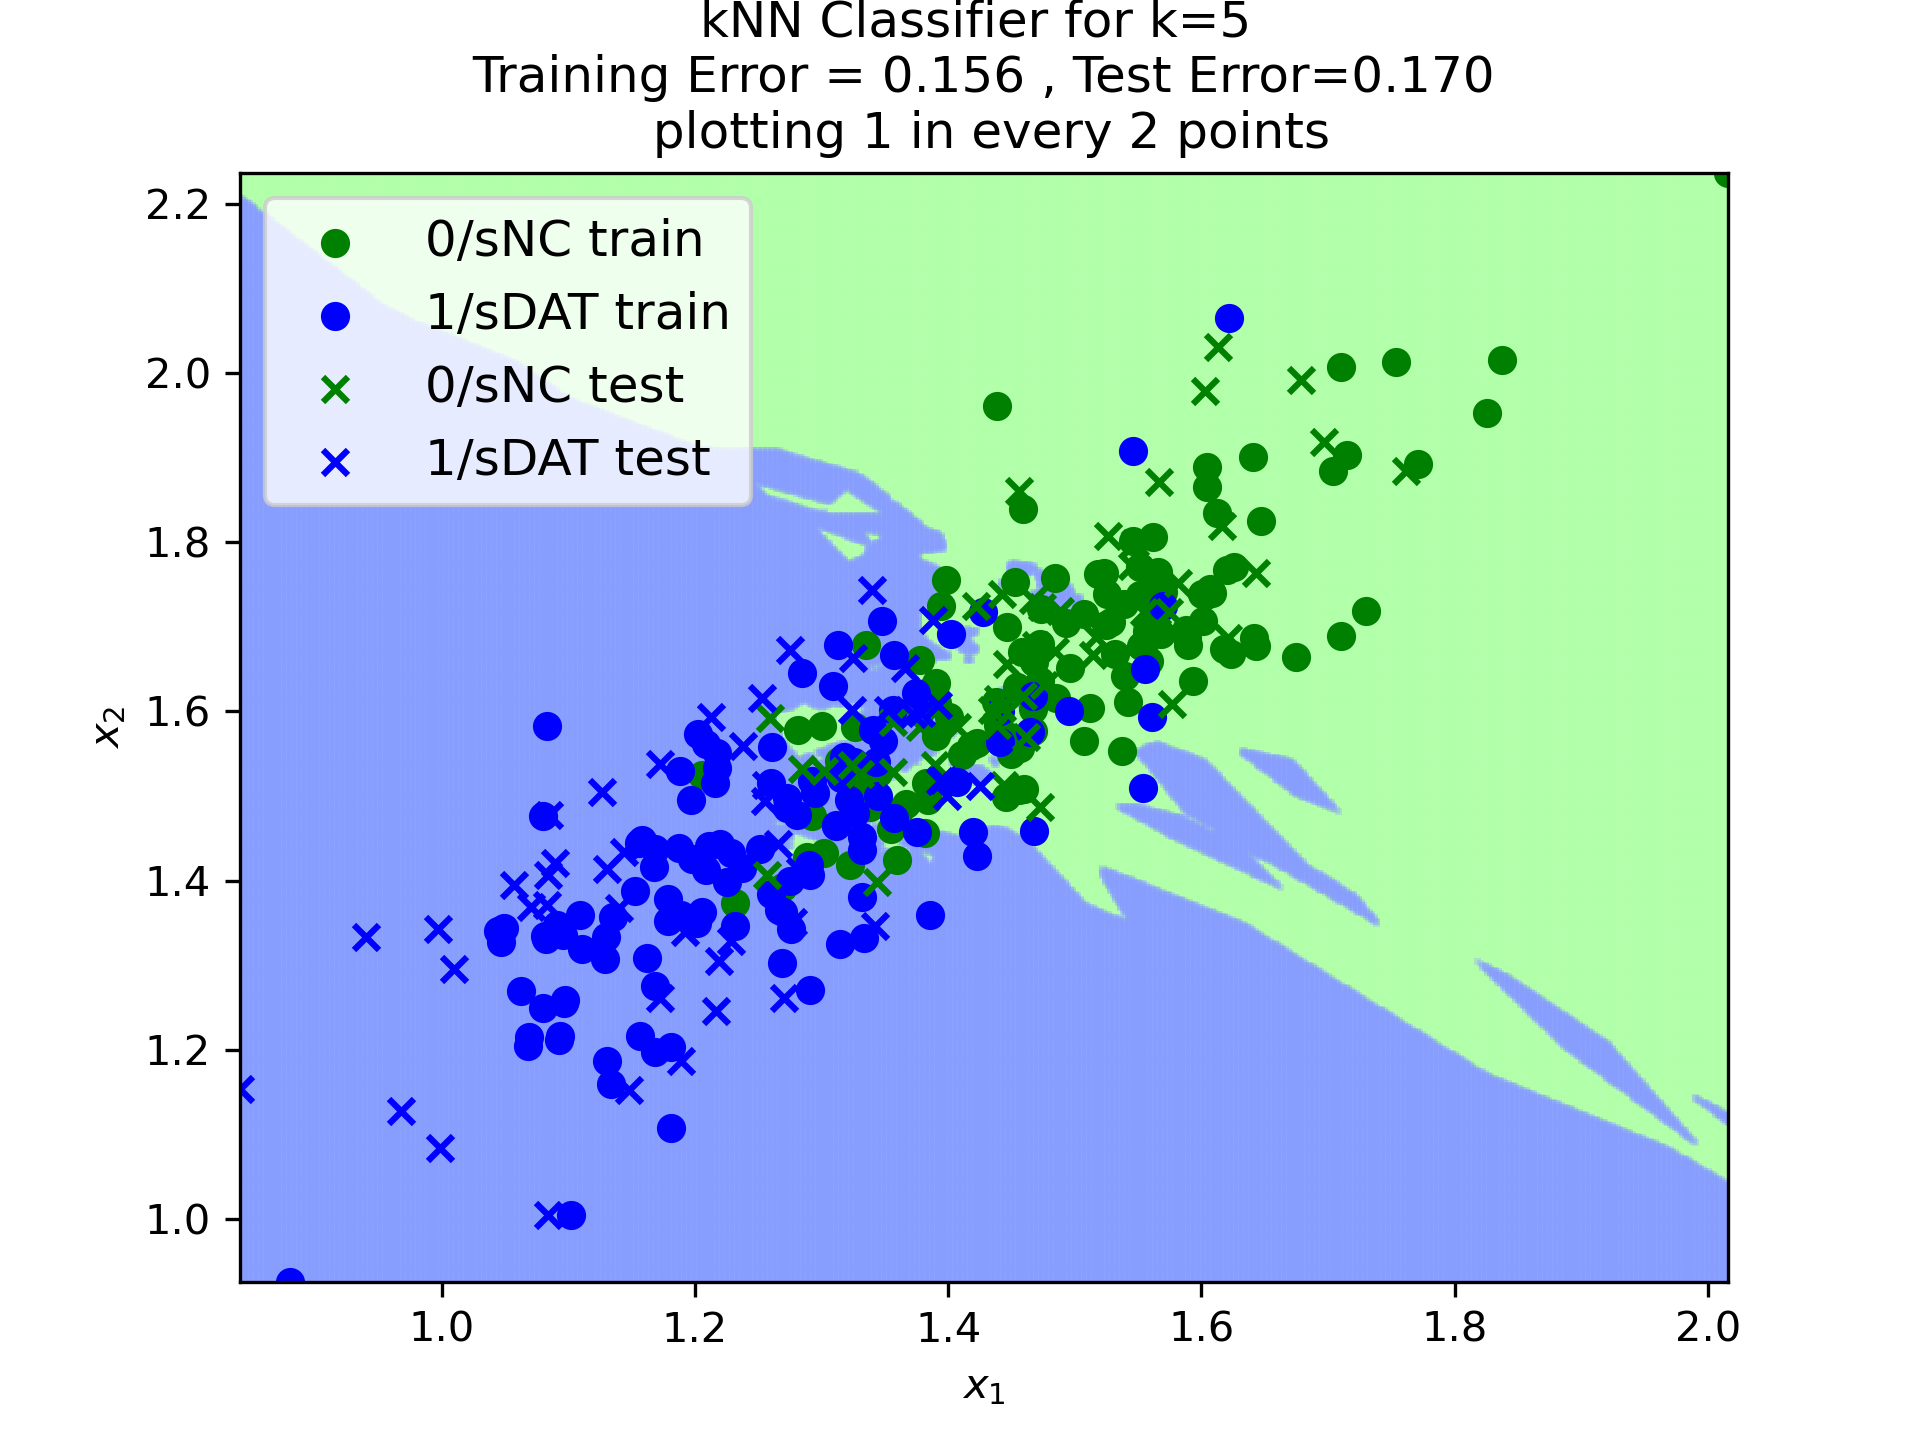
\includegraphics[width=0.95\linewidth]{Graphs/Q1_k5.png}
\captionof{figure}{Nearest Neighbor classifier for k = 5 with sDAT region in blue and sNC region colored green, with training and test data overlayed}
\label{fig:Q1k5}
\vspace{20pt}

\renewcommand{\thefigure}{4}
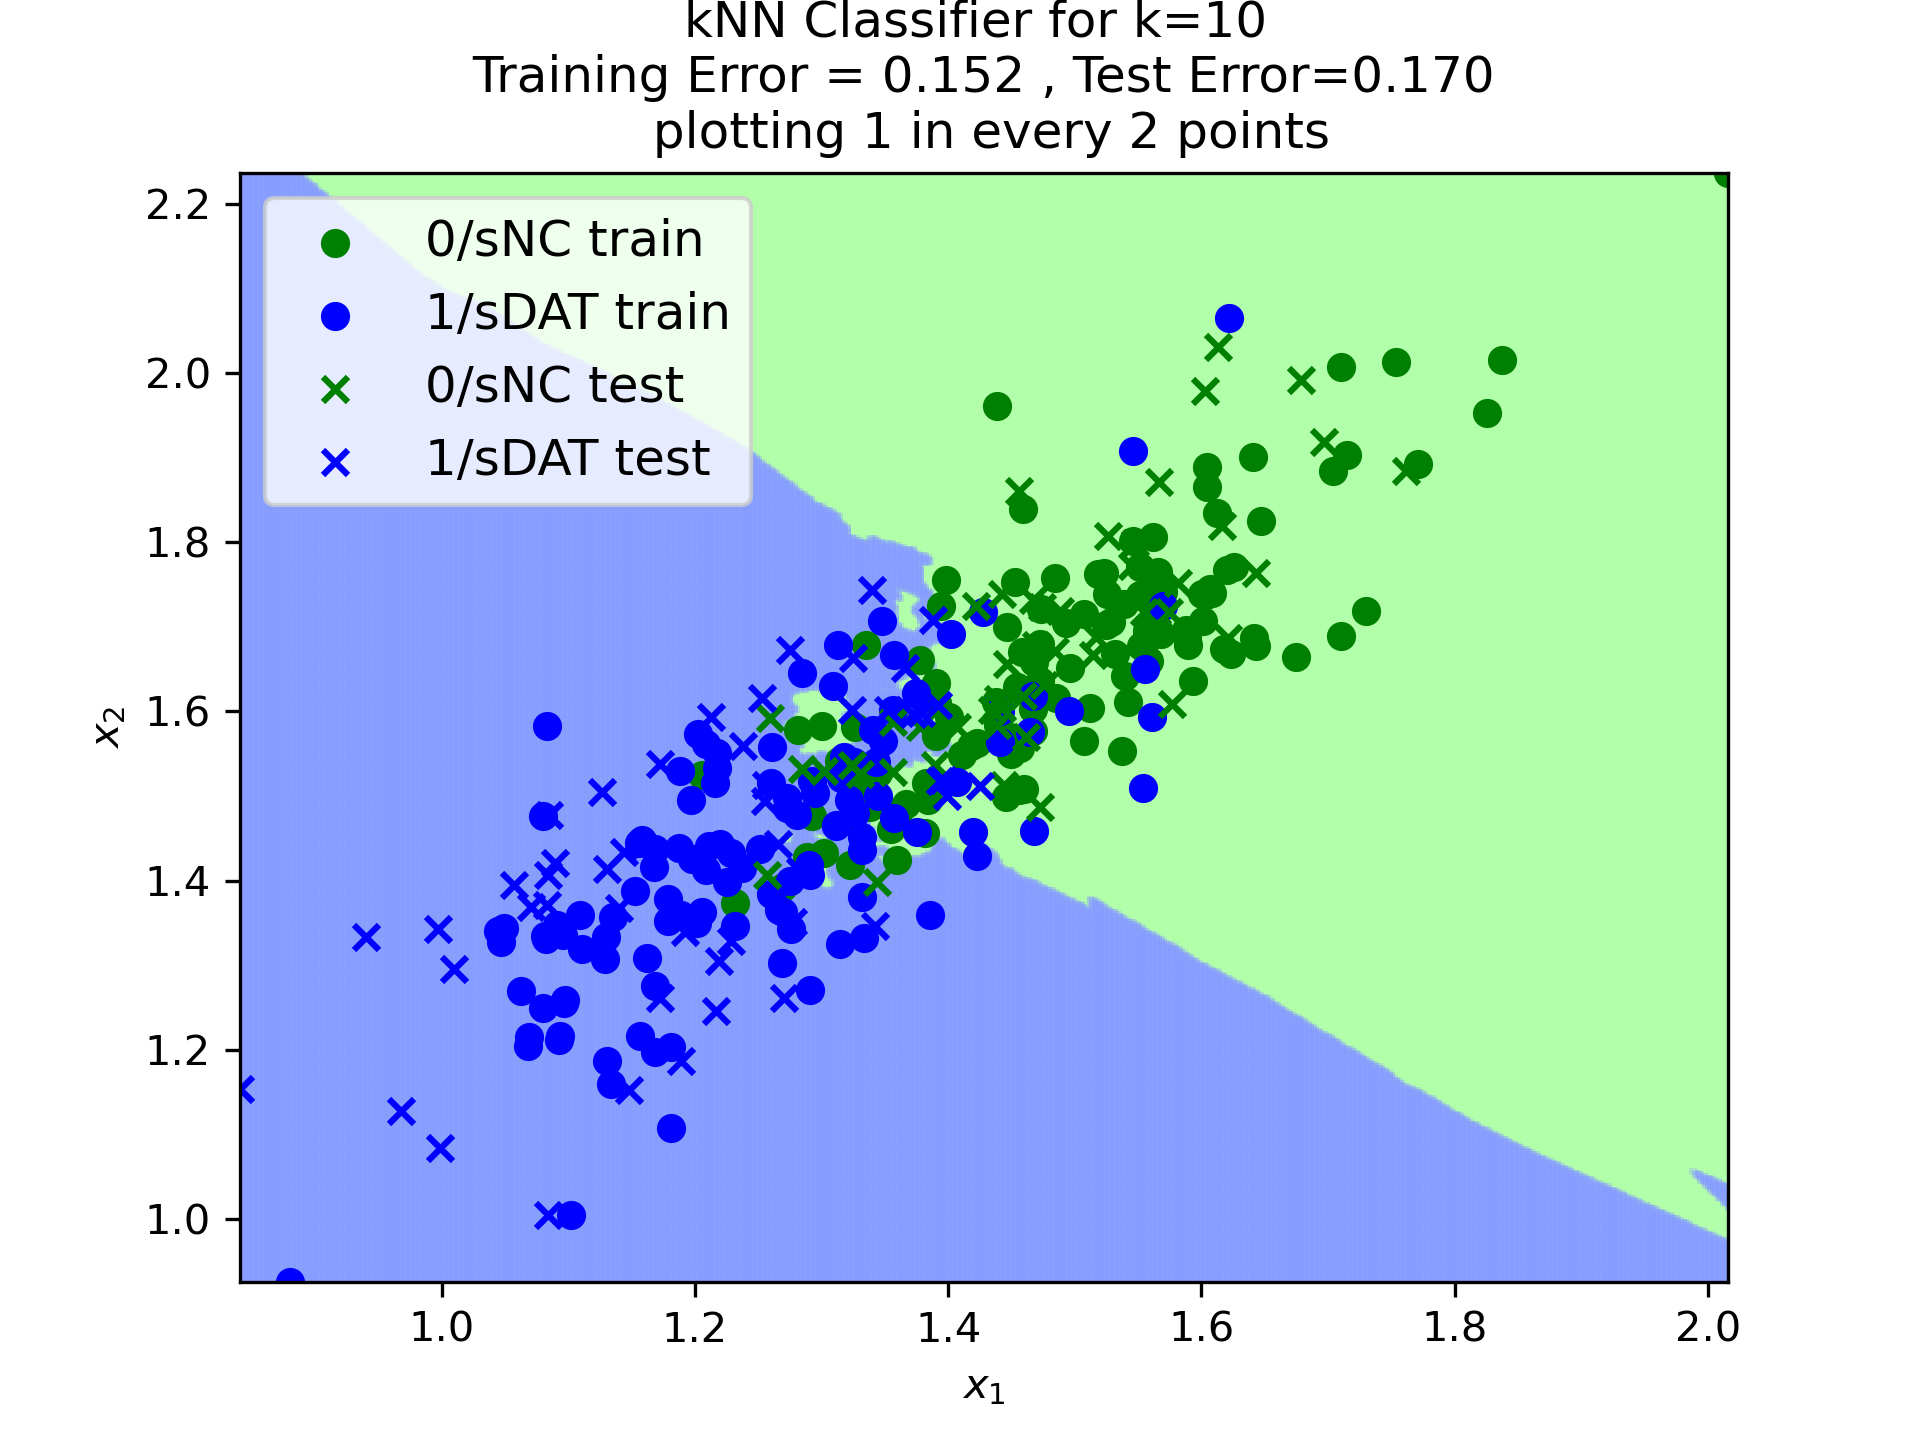
\includegraphics[width=0.95\linewidth]{Graphs/Q1_k10.png}
\captionof{figure}{Nearest Neighbor classifier for k = 10 with sDAT region in blue and sNC region colored green, with training and test data overlayed}
\label{fig:Q1k10}
\vspace{20pt}

\renewcommand{\thefigure}{5}
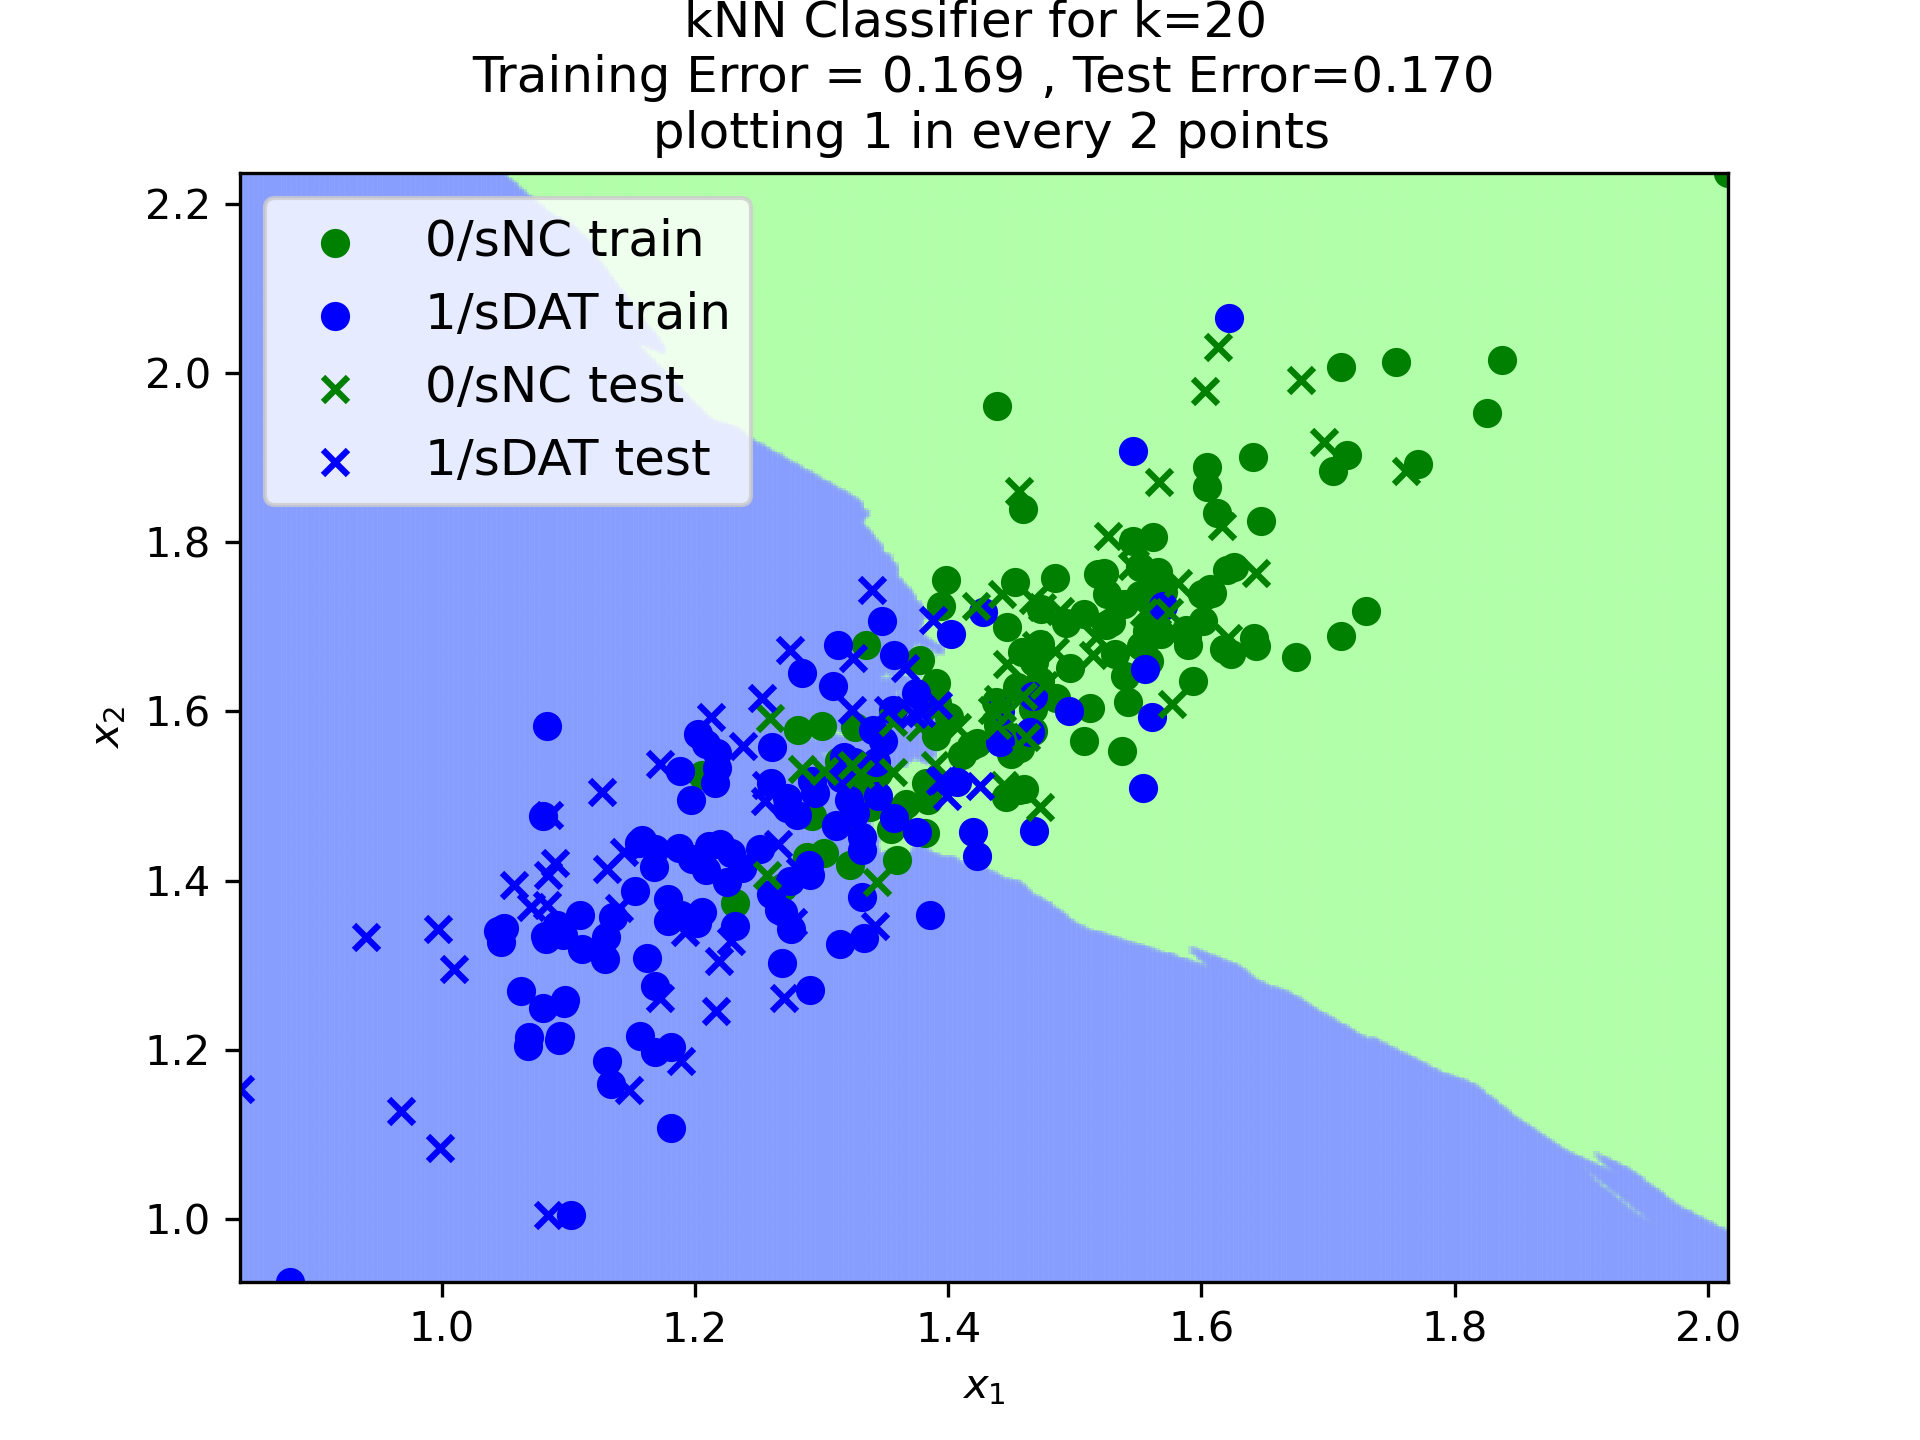
\includegraphics[width=0.95\linewidth]{Graphs/Q1_k20.png}
\captionof{figure}{Nearest Neighbor classifier for k = 20 with sDAT region in blue and sNC region colored green, with training and test data overlayed}
\label{fig:Q1k20}
\vspace{20pt}

\renewcommand{\thefigure}{7}
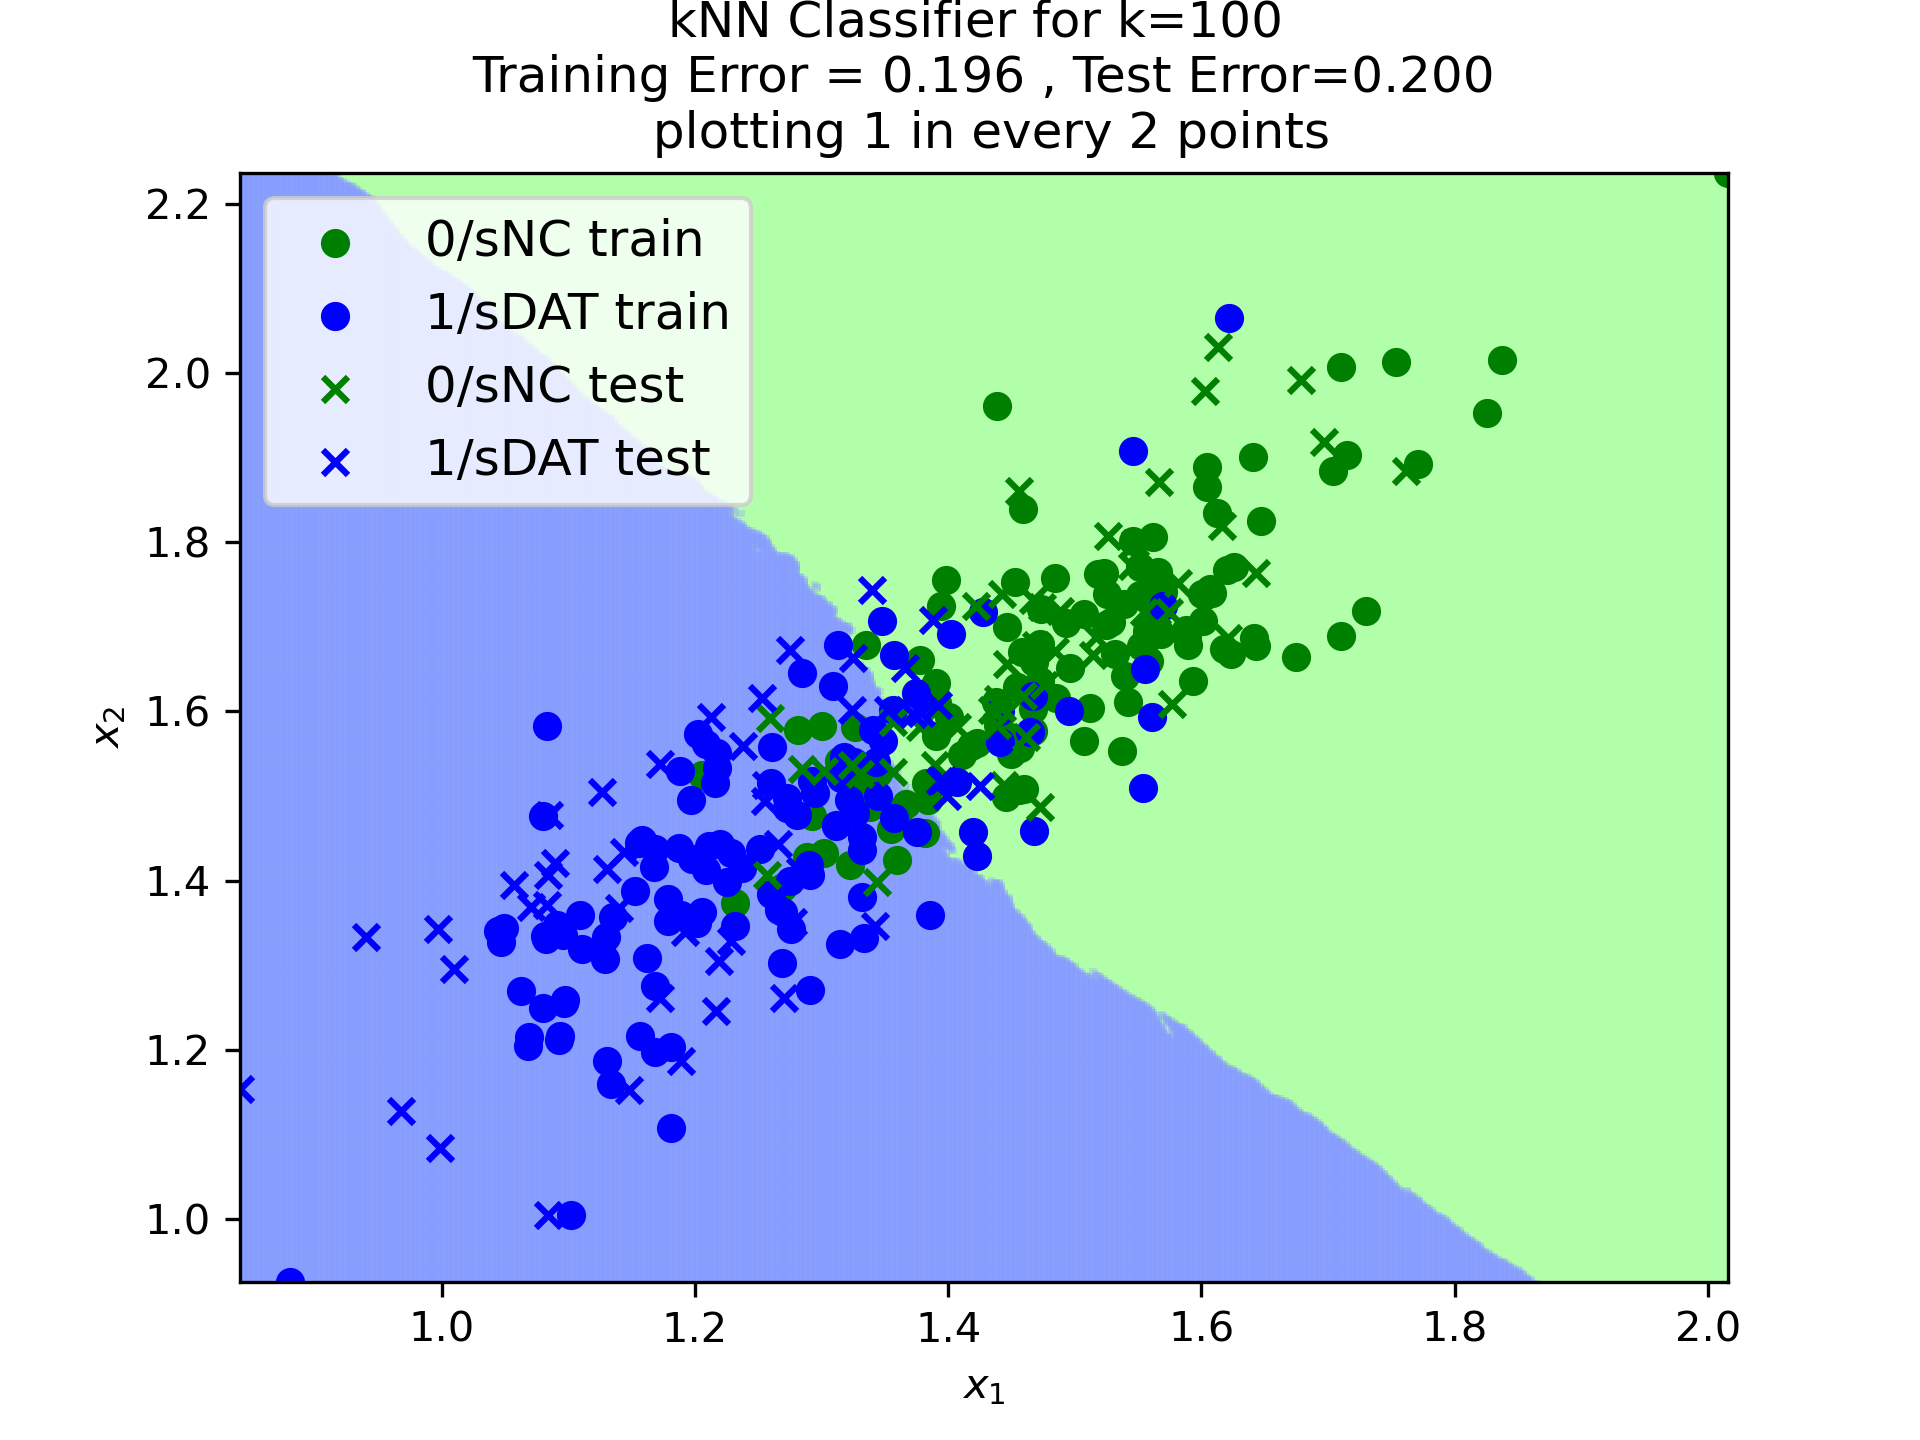
\includegraphics[width=0.95\linewidth]{Graphs/Q1_k100.png}
\captionof{figure}{Nearest Neighbor classifier for k = 100 with sDAT region in blue and sNC region colored green, with training and test data overlayed}
\label{fig:Q1k100}
\vspace{20pt}

\renewcommand{\thefigure}{9}
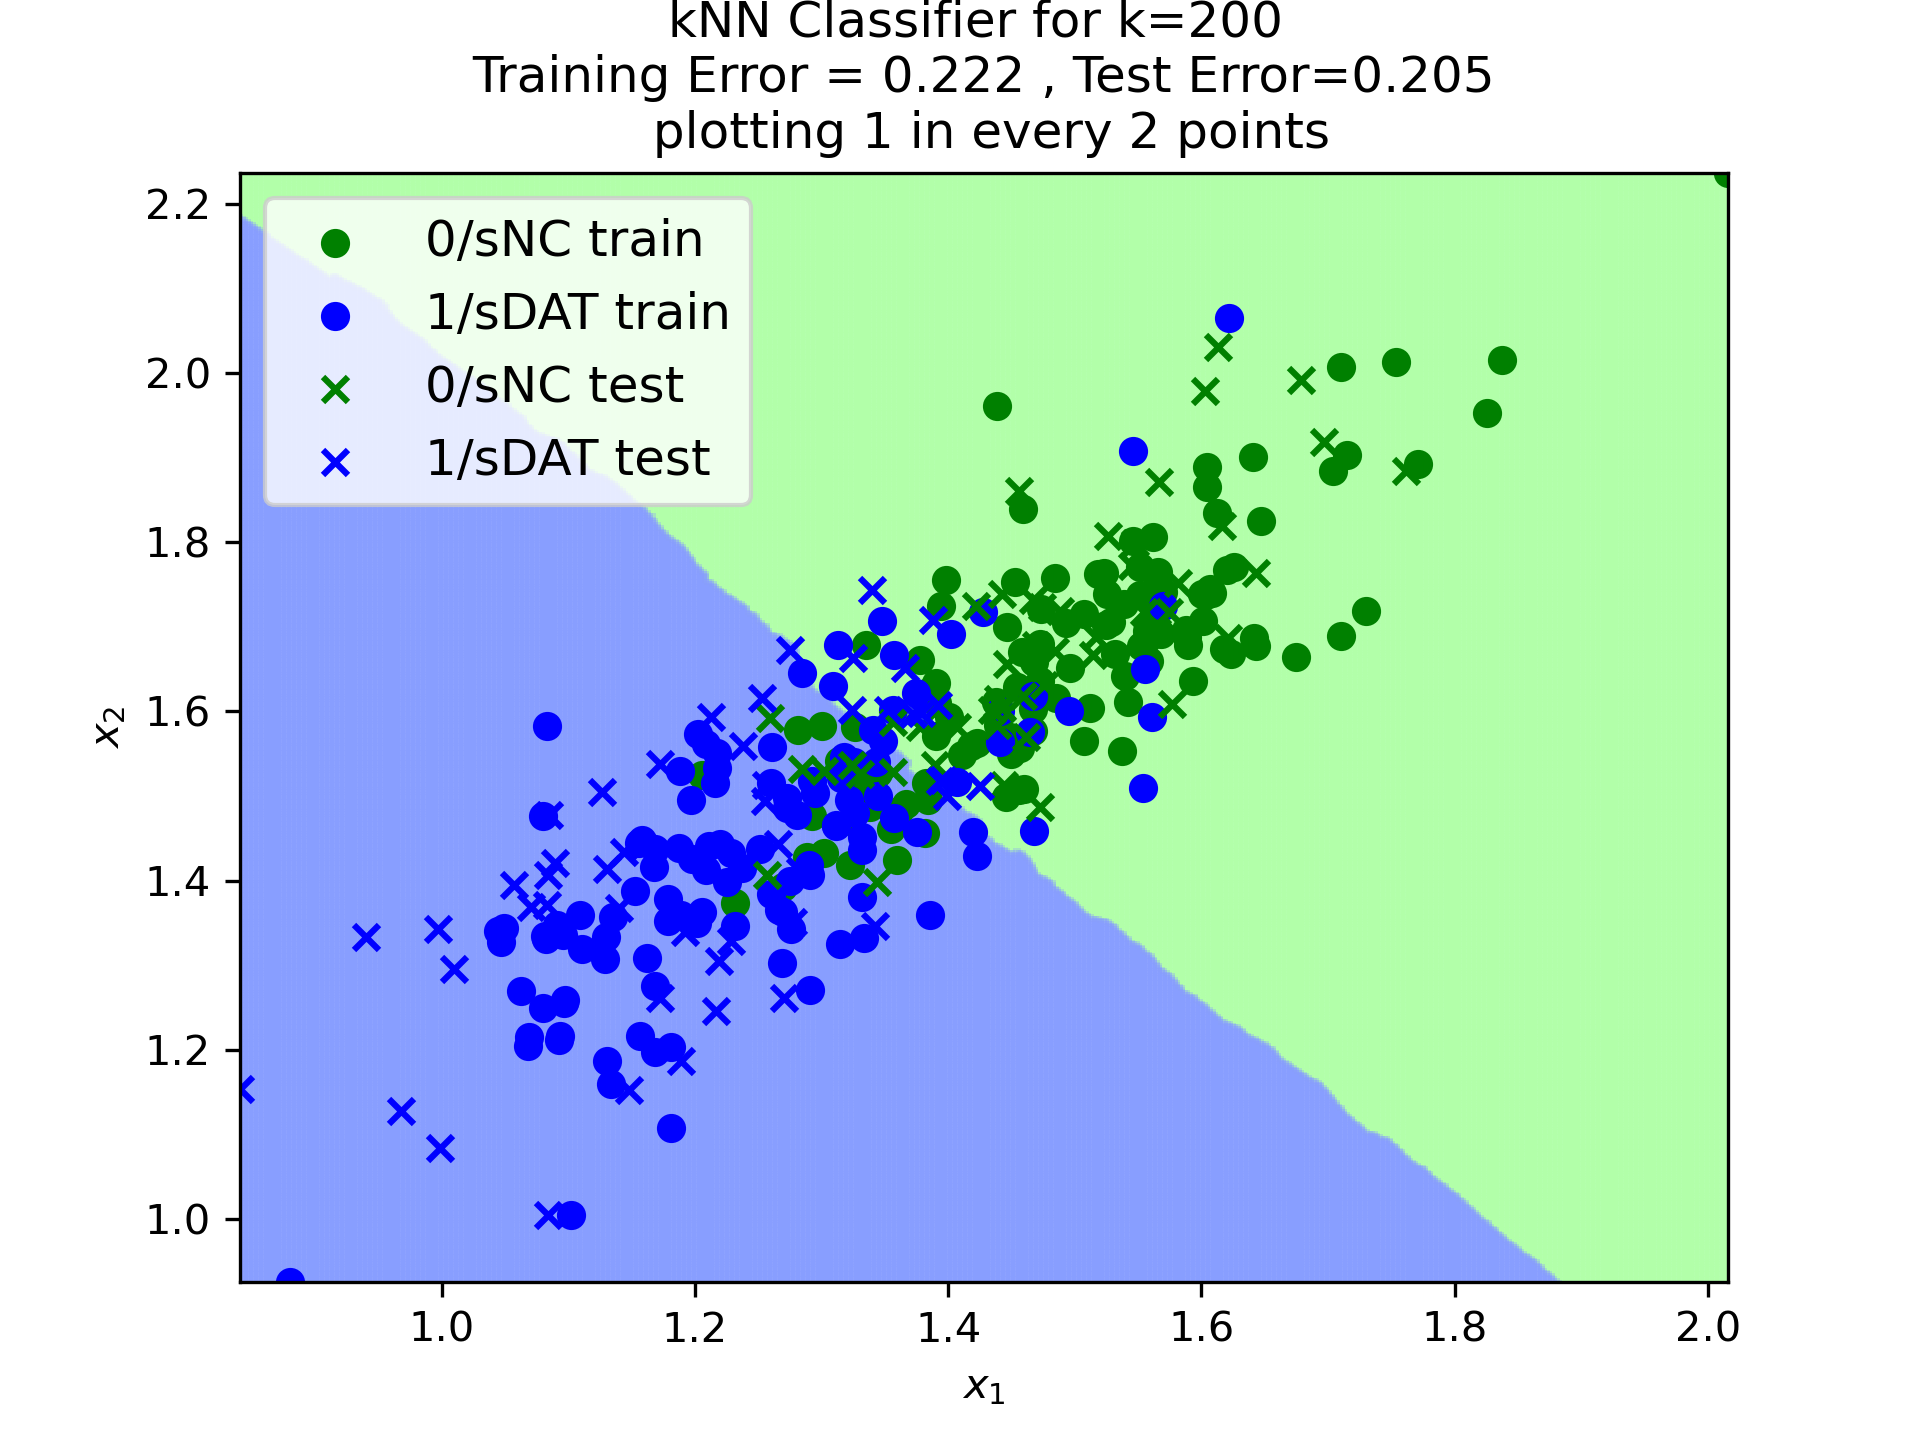
\includegraphics[width=0.95\linewidth]{Graphs/Q1_k200.png}
\captionof{figure}{Nearest Neighbor classifier for k = 200 with sDAT region in blue and sNC region colored green, with training and test data overlayed}
\label{fig:Q1k200}
\vspace{20pt}


  \vspace{2cm}


\end{paracol}

